%%
% The BIThesis Template for Bachelor Graduation Thesis
%
% 北京理工大学毕业设计(论文)第一章节 —— 使用 XeLaTeX 编译
%
% Copyright 2020 Spencer Woo
%
% This work may be distributed and/or modified under the
% conditions of the LaTeX Project Public License, either version 1.3
% of this license or (at your option) any later version.
% The latest version of this license is in
%   http://www.latex-project.org/lppl.txt
% and version 1.3 or later is part of all distributions of LaTeX
% version 2005/12/01 or later.
%
% This work has the LPPL maintenance status `maintained'.
%
% The Current Maintainer of this work is Spencer Woo.
%
% 第一章节

\chapter{算法理论}

\section{优化函数}

\subsection{梯度下降方法}

梯度下降方法是本文中主要使用的优化函数算法,它是一种用于寻找可微函数局部最小值的一阶迭代优化算法。 这个想法是在某点函数的梯度(或近似梯度)相反方向上重复执行上述步骤,因为梯度的下降方向是损失函数下降最快的方向,顺着梯度下降方向可以得到损失函数的局部最小值。相反,沿梯度方向步进将得出损失函数的局部最大值,该过程称为梯度上升。梯度下降方法包括两大类,分别是固定学习率的梯度下降算法与自适应学习率的算法。

固定学习率:

恒定学习率的代表算法有BGD、SGD、MBGD等,这三种算法的主要区别即为使用训练集中不同数量的训练数据计算损失函数的梯度。

BGD(批量梯度下降)算法主要通过对整个训练集进行损失函数计算得出最优梯度,由于对训练集的每个样本都进行了梯度计算,所以BGD可以保证梯度下降方向为全局最优方向,但是在迭代过程中需要对每个参数求偏导,且在对参数求偏导的过程中还需要对训练集遍历一次,所以BGD的问题是整个训练计算量过大导致训练成本过高,而且不能投入新数据实时更新模型。BGD伪代码如下:




通过对迭代次数nb\_epochs进行定义,我们首先计算梯度向量 params\_grad,然后沿着梯度的方向更新参数 params,其中learning rate (学习率)的作用是决定了优化过程中我们每一步迈多大。

随机梯度下降(SGD)是另一种梯度下降迭代方法,用于以合适的参数(例如可微或亚可微)优化目标函数,可以将其视为梯度下降优化的随机近似值,因为它将实际的梯度(由整个数据集计算得出)替换为估计值(由训练集随机选择子集计算得出)。与BGD相比SGD在高维优化问题中减少了计算负担,从而以较低的收敛速度实现了更快的迭代。但是由于SGD的数据是从全部数据集中随机选出,所以SGD的噪音较BGD更多,这导致了SGD的下降方向不一定是向着整体迭代最优的方向。所以SGD虽然训练速度快,但是它的缺点是训练准确度下降。

除此以外还有MBGD 方法,它的原理是每次迭代过程中利用一小批样本(mini-batch)进行计算,MBGD相比SGD可以降低参数更新时的方差从而使收敛更稳定,因为MBGD在迭代中每次使用一小批样本而不是一个样本进行梯度的计算与更新。

由于SGD的训练迭代速度更快,所以它在大数据量上有较好效果,而绝大部分梯度下降方法的优化都是基于SGD及其固有问题实现。一般而言在机器学习中,设置学习速率(步长)太高会导致算法发散,而将其设置得太低会使收敛变慢。所以从概念上讲,随机梯度下降的简单扩展就是使学习速率成为迭代次数t的递减函数ηt,从而使学习速率随着训练迭代次数增加而调整。

\subsection{自适应学习率}

自适应学习率优化算法包括Adagrad、Adadelta、RMSProp与Adam等。

Momentum算法是基于物理学中动量思想设计出的一种优化算法,由于SGD算法的学习率固定所以在收敛过程中存在震荡的问题,所以Momentum算法在梯度下降的过程中加入惯性的概念。它的主要思想是梯度的下降的方向由两个因素共同决定,分别是由当前点的梯度方向决定,还由此前的累积的梯度决定,在当前梯度方向与历史梯度一致时,会增强该方向的梯度从而加快收敛。

Momentum算法虽然没有改变学习率但是从效果上讲起到了加快收敛的作用,并成为了Adam算法的基础。

在实验过程中,我主要使用了Adam(自适应矩估计)优化函数进行梯度计算以及更新。Adam\cite{kingma2014adam}于2015年由Diederik Kingma以及Jimmy Ba在ICLR上提出,根据作者所述,Adam是对Adaptive Gradient Algorithm (AdaGrad)以及Root Mean Square Propagation (RMSProp)的优化器的扩展。AdaGrad算法核心在于可变的参数学习率,具体而言,频繁出现的参数AdaGrad使用更小的更新速率,对于不频繁出现的参数使用更大的更新速率。AdaGrad改善了对稀疏梯度问题的优化性能,在自然语言与计算机视觉等领域的深度学习模型中有着不错的效果。

RMSProp算法则是对AdaGrad的进一步优化,它引入了一个衰减系数r并且此系数在每个训练epoch都按一定比例衰减,从而解决了AdaGrad在深度学习中可能过早结束的问题。RMSProp的第一个参数实际上与AdaGrad的第一个更新向量相同,同时RMSProp还引入了另一个参数即为学习率除以平方梯度的指数衰减平均值。RMSProp算法适合处理非平稳的目标,对于RNN等网络的效果很好。

在Adam算法中,Adam除了像RMSProp中那样根据平均第一矩(均值)调整参数学习率,同时也使用了梯度第二矩(无中心方差)的平均值(有偏方差)。具体来说,该算法计算梯度和平方梯度的指数移动平均值,并且使用两个超参数beta1和beta2控制这些移动平均值的衰减率。在移动过程中,均质的初始值和beta1、beta2的超参数的值接近1,此时的误差接近0,接下来通过计算带变差估计与偏差修正后的估计进行对比从而使得优化函数得到提升。Adam本质上是带有动量项的RMSprop,Adam的主要优点在于经过偏置校正后,每一次迭代学习率都有确定范围,使得参数比较平稳。经过实验证明Adam在实践中比上述优化算法有更好的表现。

Adam的主要参数包括${\alpha}$(学习率)、${\beta}_{1}$(一阶矩估计的指数衰减率)、${\beta}_{2}$(二阶矩估计的指数衰减率)、${\epsilon}$。



\section{目标函数}

目标函数在广义上指经验函数+结构化函数,而训练模型的目的在于使经验风险与结构化风险最小化,经验风险即为我们在训练机上训练所得到的模型准确率高低,对于给定的训练集而言,对于模型拟合的越好那么经验风险(预测失败)的概率越低,但是需要注意的是模型的经验风险并非越低越好,因为在经验风险低的情况下虽然模型在训练集的准确率变高,但是模型可能因为拟合好而变得更为复杂从而缺少泛化能力,所以也引入了结构风险的概念,结构风险即为模型的复杂程度,降低结构化风险要采取奥坎姆剃刀的原则,在模型的准确率与模型的复杂程度上进行取舍。过高的结构复杂度可能导致过拟合的情况,而过低的复杂度将导致模型训练不足产生误差。而在我们的系统中由于推荐系统的衡量指标不仅仅是误差函数,同时也包括准确率、召回率以及roc-auc curve等,所以在这里以不包括结构化objective function定义目标函数。

对于一个优化问题而言,目标函数被定义为用来评估候选集结果(即一组权重)的函数,我们可能需要最大化或者最小化目标函数,意味着我们要在候选集中寻找有着相对最高/最低的目标函数值。具体而言在神经网络中,我们希望使误差最小化,在这种情况下,目标函数也常被称为损失函数或代价函数(cost function),对于一个模型而言,损失函数的意义在于将一个复杂的系统所有优缺点降低为一个标量值,从而可以对候选解决方案进行排名和比较\cite{NeuralSmithing}。在这个系统中主要使用的损失函数包括mlogloss、binary-crossentropy等。

首先目标函数分为两大类,一类是用于回归问题,另一类是用于分类问题,由于我们的系统主要实现的是分类功能,所以在这里着重介绍分类相关的目标函数。

\subsection{均方误差}

均方误差指预测值与实际观察值之间的平方差的平均值。如果预测值和真实值相差较大,此预测会因为平方项的存在将误差以平方扩大而受到较大惩罚。另外,MSE具有良好的数学特性,使得这个函数可以更有效地对梯度进行更新迭代。

\subsection{最大似然估计}

虽然有许多目标函数都可用于估计神经网络中一组权重的误差,但是我们倾向于使用一种能够将候选权值的空间映射到平滑(高维)空间上,使得优化算法可以通过对模型权重进行迭代更新来更合理地进行权值修正。最大似然估计(MLE)是用于从历史训练数据中找到合适参数最佳统计估计的推理框架,这种方法正是我们正在尝试在神经网络的修正工作上使用的。Neural Networks For Pattern Recognition中曾指出:Maximum likelihood seeks to find the optimum values for the parameters by maximizing a likelihood function derived from the training data.(最大似然估计是通过计算训练集得到的似然函数而对参数进行优化) \cite{NeuralNetworkforPatternRecognize}.最大似然估计损失函数是评估训练目标和模型预测值分布差异的方法。使用最大似然估计的好处是随着训练数据的增长,模型参数预估的效果会提升,这是由于最大似然估计具有统计学中一致性的特点\cite{DeepLearning2016}。

\subsection{交叉熵}

从技术上讲,交叉熵(Cross-Entropy)概念来自于信息理论,并以“位”为单位。交叉熵是建立在最大似然估计的基础之上的,我们希望通过使用交叉熵函数优化模型权重以最小化模型预测的概率分布以及训练集的概率分布之间的差异。除此以外,在最大似然估计的基础上使用高斯分布作为目标,MSE也可以被理解为模型预测与目标分布之间的交叉熵。所以在实际应用中,MSE也同时被作为交叉熵的一部分用于回归问题而且在一部分分类问题的应用中也会使用MSE作为损失函数。在神经网络中,使用交叉熵损失函数的模型极大的提高了 sigmoid 和 softmax 层作为激活函数的输出神经元的效果。

对于二分类问题训练数据集中的一条数据而言,它存在一个已知的类别标签,概率为1.0,所有其他标签的概率为0.0,模型可以估计训练集中某数据属于每个列别标签的概率并且使用交叉熵来计算两个概率分布之间的差异。所以我们可以将数据标签映射到具有概率分布的随机变量上,若以P表示真实值,Q表示预测值,那么每一条数据所代表的交叉熵公式就可表示如下:



而由于对于一个特定的分类问题而言,输出结果可以用列向量y=[$y_{1}$ ,$y_{2}$ ,...,$y_{n}$]$\mathrm{T}$表示,其中当$y_{i}$为预测判定时,$y_{i}$=1其他为0。此时$p_{j}$ = $y_{j}$,那么交叉熵公式可以如下表示:




那么对于具有N个样本的损失函数计算而言,它可以表示为如下形式:



$y_{i}$表示样本$i$的label,正类为1,负类为0

$p_{i}$为样本i预测为正的概率

实际上在二分类问题中的交叉熵损失函数也被称为logloss。

多分类问题本质上是对二分类问题的扩展,多分类问题的公式可以表示如下:




其中M代表类别的数量

$y_{ic}$代表指示变量,如果该类别和样本$i$的类别相同就是1,否则是0;

$p_{ic}$为对于观测样本$i$属于类别$c$的预测概率。

在一个二分类问题中交叉熵的公式如上。




\section{推荐系统评价指标}

精确率、精确率和召回率是在推荐系统中对模型进行评价的几个重要指标,在这里首先要引入TP、FP、FN与TN的概念。TP即为True Positives,也就是将正类判断正确,FP即为负类判断为正类,FN也就是正类判断为负类,TN即为负类判断为负类,准确率的公式即可如下表示:
\begin{equation}
  acc = \frac{TP + TN}{Total}
\end{equation}

\subsection{精确率}

精确率是指所有判定为正类的样本中,真实正类所占比例,公式如下:
\begin{equation}
  pec = \frac{TP}{TP + FP}
\end{equation}

\subsection{召回率}

召回率(真阳性率),即指所有真实正类中,判定为正类的比例,公式如下:
\begin{equation}
  rec = \frac{TP}{TP + FN}
\end{equation}

\subsection{${\kappa}$系数}

除此以外还可以使用${\kappa}$系数衡量分类效果。${\kappa}$系数是进行检验一致性的重要指标,对于分类问题而言,一致性即指模型预测结果与实际分类结果之间的差异,${\kappa}$系数是通过对混淆矩阵计算而得到的,取值在[-1, 1]之间,一般${\kappa}$系数的值为正,当${\kappa}$系数落在[0, 0.20]之间时,模型的一致性极低,[0.21, 0.40]之间时,模型的一致性一般,[0.41, 0.60]之间时,模型的一致性中等,[0.61, 0.8]之间时,模型的一致性较高,[0.81, 1.0]之间时,模型的一致性极高。${\kappa}$系数的计算公式如下:
\begin{equation}
  {\kappa} = \frac{p_{0} - p_{e}}{1 - p_{e}}
\end{equation}

其中$p_{0}$即为accuracy,$p_{e}$为
\begin{equation}
  p_{e} = \frac{\sum_{i} \text{第\emph{i}行元素之和}\times\text{第\emph{i}列元素之和}}{(\sum \text{矩阵所有元素})^2}
\end{equation}


即各类别对应的“实际数量与预测数量的乘积”的总和再与样本总数的平方相除。

\subsection{ROC-AUC曲线与AUC值}

ROC曲线为FPR与TPR之间的关系曲线,其中FPR指假阳性率,也就是所有负样本中分类器将负样本预测为正样本的比例,而TPR指真阳性率,也就是Recall值,ROC曲线的定义为以FPR作为x轴TPR作为y轴的曲线,这个组合总FPR对TPR即可理解为代价对收益,通过改变不同的阈值可以得到一系列TPR与FPR并绘制出ROC曲线,而AUC值即是指ROC曲线与坐标轴围成区域的面积,AUC值反映了分类器对样本的排序能力。FPR与TPR的公式如下所示。
\begin{equation}
  TPR = \frac{TP}{TP + FN}
  \qquad
  FPR = \frac{FP}{FP + TN}
\end{equation}




\section{聚类算法}

在本文中使用聚类算法的目的主要是进行特征工程,分别使用了HDBSCAN、Spectral Clustering与K-Means几种不同的算法来进行聚类结果比较。其中KMeans是一种常用的机器学习算法,不做赘述。

\subsection{谱聚类}

谱聚类是一种来源于图论的算法,它将数据看做空间中的点,这些点之间可以用边连接起来。连接点的边的权值大小和两个点之间的距离有关,距离越近权值越高,距离越远权值越低。通过对所有数据点组成的图进行切图,目标是使得切图后不同子图间边的权重和尽可能的低,子图内边的权重和尽可能的高而实现聚类。
谱聚类通过这些图上的点映射到一个低维易于分离的空间从而逐渐实现距离度量并最终聚类。 谱聚类使用来自图形或数据集的特殊矩阵(即距离矩阵(Affinity Matrix),度矩阵(Degree Matrix)和拉普拉斯矩阵(Laplacian Matrix))的特征值(频谱)中的信息。谱聚类是一种优秀的算法,较KMeans相比谱聚类对数据分布适应性更强,聚类效果也更优秀,同时计算量也小很多。

\subsection{HDBSCAN}

DBSCAN是一种常用的基于密度的聚类方法,HDBSCAN相比于DBSCAN将传统的密度聚类转换为分层聚类扩展了DBSCAN,然后基于聚类稳定性使用平面聚类提取技术提高了聚类效果的鲁棒性,最为重要的是基于密度的聚类算法可以通过指定最小生成类簇的大小自动推荐最优簇类结果生成最优聚类簇数k,同时HDBSCAN相比于DBSCAN不用选择人工选择领域半径R和MinPts。

\section{推荐算法}

选择合适的推荐算法是一个推荐系统成功与否的关键,对于这个问题我们主要使用了3种不同的推荐算法,分别涵盖了最基础的机器学习算法--贝叶斯分类器,推荐领域大显身手的决策树模型--XGBoost以及基于深度学习并且可以摆脱手动特征工程困扰的典型模型--DeepFM。

\subsection{贝叶斯分类器}

贝叶斯分类器是以贝叶斯定理为基础的简单概率分类器,它通过数据分布的先验概率利用贝叶斯公式计算后验概率,我们在实验中使用了三种不同的朴素贝叶斯分类器,分别是高斯、伯努利以及多项式。它们的区别是在使用最大似然估计对数据进行估计时假设的数据分布概率函数不同。

\subsection{XGBoost}

XGBoost是使用梯度提升(Gradient Boosting)的基于决策树的集成机器学习算法。在涉及非结构化数据(图像,文本等)的预测问题中,人工神经网络往往胜过所有其他算法或框架。但是,当涉及中小型结构化/表格数据时,基于决策树的算法目前被认为是同类中最好的。

虽然XGBoost与梯度提升算法一样,都是使用Boosting算法的思想将许多弱分类器如CART回归树模型等集成在一起在梯度下降的优化下形成一个强分类器,但是XGBoost通过对GBM(Gradient Boosting Machine)进行改进从而提升了算法性能,具体的提升可以分为两大方面,分别是性能优化以及算法优化。

XGBoost的系统性能优化如下:

\begin{enumerate}
  \item 并行化: XGBoost通过并行计算来实现树的构建过程。以传统的决策树构造过程为例,它包括内外两个循环,外层循环用于枚举一棵树的叶子节点构造,内存循环用于特征计算。循环嵌套限制了算法的并行化能力,因为如果不完成内部循环(计算量更大),就无法启动外部循环。因此交换内外层循环的顺序可以减少运行时间,循环的交换通过初始化多个运行在所有实例上的扫描与排序线程实现。交换通过并行计算减少算法运行时间。
  \item 剪枝算法: 梯度提升框架中决策树分裂的停止准则本质上是贪婪的,并且取决于分裂时的负损失准则。 XGBoost使用“max\_depth”参数代替GBM的分裂标准,然后开始向后剪枝。这种深度优先的方法显著提高计算性能。
  \item 存储优化: XGBoost通过在每个线程中分配内部高速缓冲区(Cache)来存储梯度统计信息来实现的。同时使用诸如“out-of-core”等方法增强对超大数据帧(DataFrame)的处理,并且进一步优化了内存和磁盘空间使用。
\end{enumerate}

算法优化如下:

\begin{enumerate}
  \item 正则化: XGBoost通过使用L1和L2正则化参数计算模型的结构复杂度并防止过拟合。
  \item 稀疏感知: 为解决稀疏特征问题,为每个树节点选择默认方向,如果某个样本对应特征缺失,直接划入默认方向。\cite{XGBoost原理解析}
  \item 加权分位数: XGBoost通过加权分类数算法(Weighted Quantile Sketch)寻找最优分裂点。
  \item 交叉验证: 算法通过内置交叉验证来获取最优参数并防止过拟合。
\end{enumerate}

\subsection{DeepFM}

CTR预测大规模应用的算法最初主要是SVM和LR,但是LR/SVM这样的线性模型无法建模非线性的特征交互,于是需要手工进行特征交叉或组合,而这个过程是复杂而且需要大量专业人员的参与;为了弥补LR/SVM无法处理非线性特征交互的问题,因子分解机([Factorization Machine](https://tech.meituan.com/2016/03/03/deep-understanding-of-ffm-principles-and-practices.html))这种方法被提出并得到大规模应用。

FM的模型由Konstanz大学Steffen Rendle于2010年提出,旨在解决稀疏数据下的特征组合问题。在CTR推荐过程中,主要存在三类数据,分别是用户的特征、广告的特征和上下文特征,这些特征很多是离散的类别特征,而这些离散的特征在使用one-hot encoding后将使特征空间急剧增大,而且变得稀疏,稀疏矩阵使得参数的计算变得困难。为了解决上述问题,FM的做法是通过矩阵分解的方法将评分矩阵分解为用户矩阵和商品矩阵,其中用户和商品都可以使用隐向量进行表示[8](http://www.cs.cmu.edu/~wcohen/10-605/2015-guest-lecture/FM.pdf);如我们将User表示为一个二维向量,同时将Item表示为二维向量,那么两个向量的点积就是User对Item的打分,如下图所示。





类似地,所有二次项参数 wij 可以组成一个对称阵 **W**(为了方便说明FM的由来,对角元素可以设置为正实数),那么这个矩阵就可以分解为 **W**=**V**T**V**,**V** 的第 j 列便是第 j 维特征的隐向量。换句话说,每个参数 wij=⟨**v**i,**v**j⟩,这就是FM模型的核心思想。因此,FM的模型方程为(本文不讨论FM的高阶形式)




FM的训练复杂度为O(kn)级别,可以在线性时间对新样本进行预测。FM通过给单独的特征引入低维稠密隐向量减少了二阶特征交互的参数,并且在这个过程中实现了信息共享,从而使稀疏特征向量的学习更加容易泛化。理论上FM可以建模二阶以上的特征交互,但是由于二阶以上的参数数量将会急剧增加而且更高维的特征交互可以使用DNN、DCN等神经网络模型实现,所以一般上只用二阶的模型。

但是由于FM模型也存在特征无法区分的问题,比如对于奖学金推荐系统而言数据的成绩特征与总学分的组合与论文的发表数量和论文的所属期刊的组合是潜在同样意义的,所以FM特征无法捕捉这样的差异,那么又提出了FFM模型,FFM即为Field-aware Factorization Machines,它在FM模型的基础上引入了Field的概念,对于其中的每一维特征,都属于一个特定的Field,Field与Feature之间存在一对多的关系。具体的实现上看,由一个Categorical feature one-hot出的多个类别特征属于同一个域(Field),而连续的特征不需要进行one-hot自己作为一个单独的域存在。[FFM的公式](https://www.csie.ntu.edu.tw/~cjlin/papers/ffm.pdf)如下:





其中x是n维特征向量,f1 f2代表j1 j2对应的field,j1 j2分别是特征向量中的两个特定index的值。FM和FFM对比而言,FM只有一个代表特征的向量,而FFM有一个代表特征向量和一个代表域的向量,也就意味着同一特征,要和不同的 fields 进行组合的时候,会用不同的embedding,因而FFM参数更多。对于一个vector的特征,现在拓成 F 个 vector,只要跟它任意组合,就有一个 vector 来代表,这就是 FFM 的基本思想。

可以看到无论是FM或是FFM,都是对两个特征进行的特征组合,那么如果有更高阶的特征组合,就需要更复杂的模型进行训练,随着深度神经网络的发展,研究发现可以使用多层的网络结构进行更好的高阶特征表示,从而学习高阶的非线性关系。而深度神经网络为代表的模型分化出了两种发展思路,一种是并行结构,一种是串行结构。





对于深度神经网络而言,都是首先将特征输入进行embedding后连接隐层进行预测,这一部分是一个公有结构,而另一个公有结构为上述介绍的FM Function,负责学习模型的二阶特征组合。串行与并行模型的区别就在于FM和DNN的关系是并行(FM与DNN同样接受embedding层的输入后将两者结果进行融合)或是串行(FM先进行二阶特征组合后将结果输入DNN进行更高阶组合)。

并行结构的代表模型有Wide \& Deep、DeepFM、NeuralFFM、DeepFFM

串行结构的代表模型有DeepCross、xDeepFM

首先提出的并行结构为Wide \& Deep,它于2016年由Google发布,它分为两个部分,分别是Wide部分以及Deep部分,其中Wide部分的作用是通过交叉特征实现高效的记忆能力,达到准确推荐的目的,使用LR等广义线性模型实现特征交叉。Deep部分则是一个前馈神经网络模型,由于基于嵌入的模型(如FM与DNN)能将输入转化为一个低维稠密向量从而获得了一定的泛化能力,减轻了特征工程的负担。embedding得到的向量作为Deep部分第一层隐藏层的输入并经过多层隐藏层厚并根据得到的loss进行训练。此模型同时学习了低阶特征与高阶特征并且在输出层对上述Deep以及Wide的结果进行加权求和,在Google Play离线测试以及在线A/B测试中都取得了超越Deep或Wide的效果。但是Wide模型存在需要手工特征处理的情况,为了解决这一问题,华为联合哈尔滨工业大学提出了一种改进模型--DeepFM。

DeepFM结合了FM和Wide \& Deep的特点,并通过共享FM和DNN的Embedding来减少参数量和共享信息,并且通过引入FM克服了手工特征处理的障碍。针对高维稀疏输入特征,DeepFM采用Word2Vec的词嵌入思想,把高维稀疏的向量映射为相对低维且向量元素不为零的空间向量。DeepFM的网络结构如\ref{DeepFM结构图}所示。
\begin{figure}[htb]
  \vspace{13pt} % 调整图片与上文的垂直距离
  \centering
  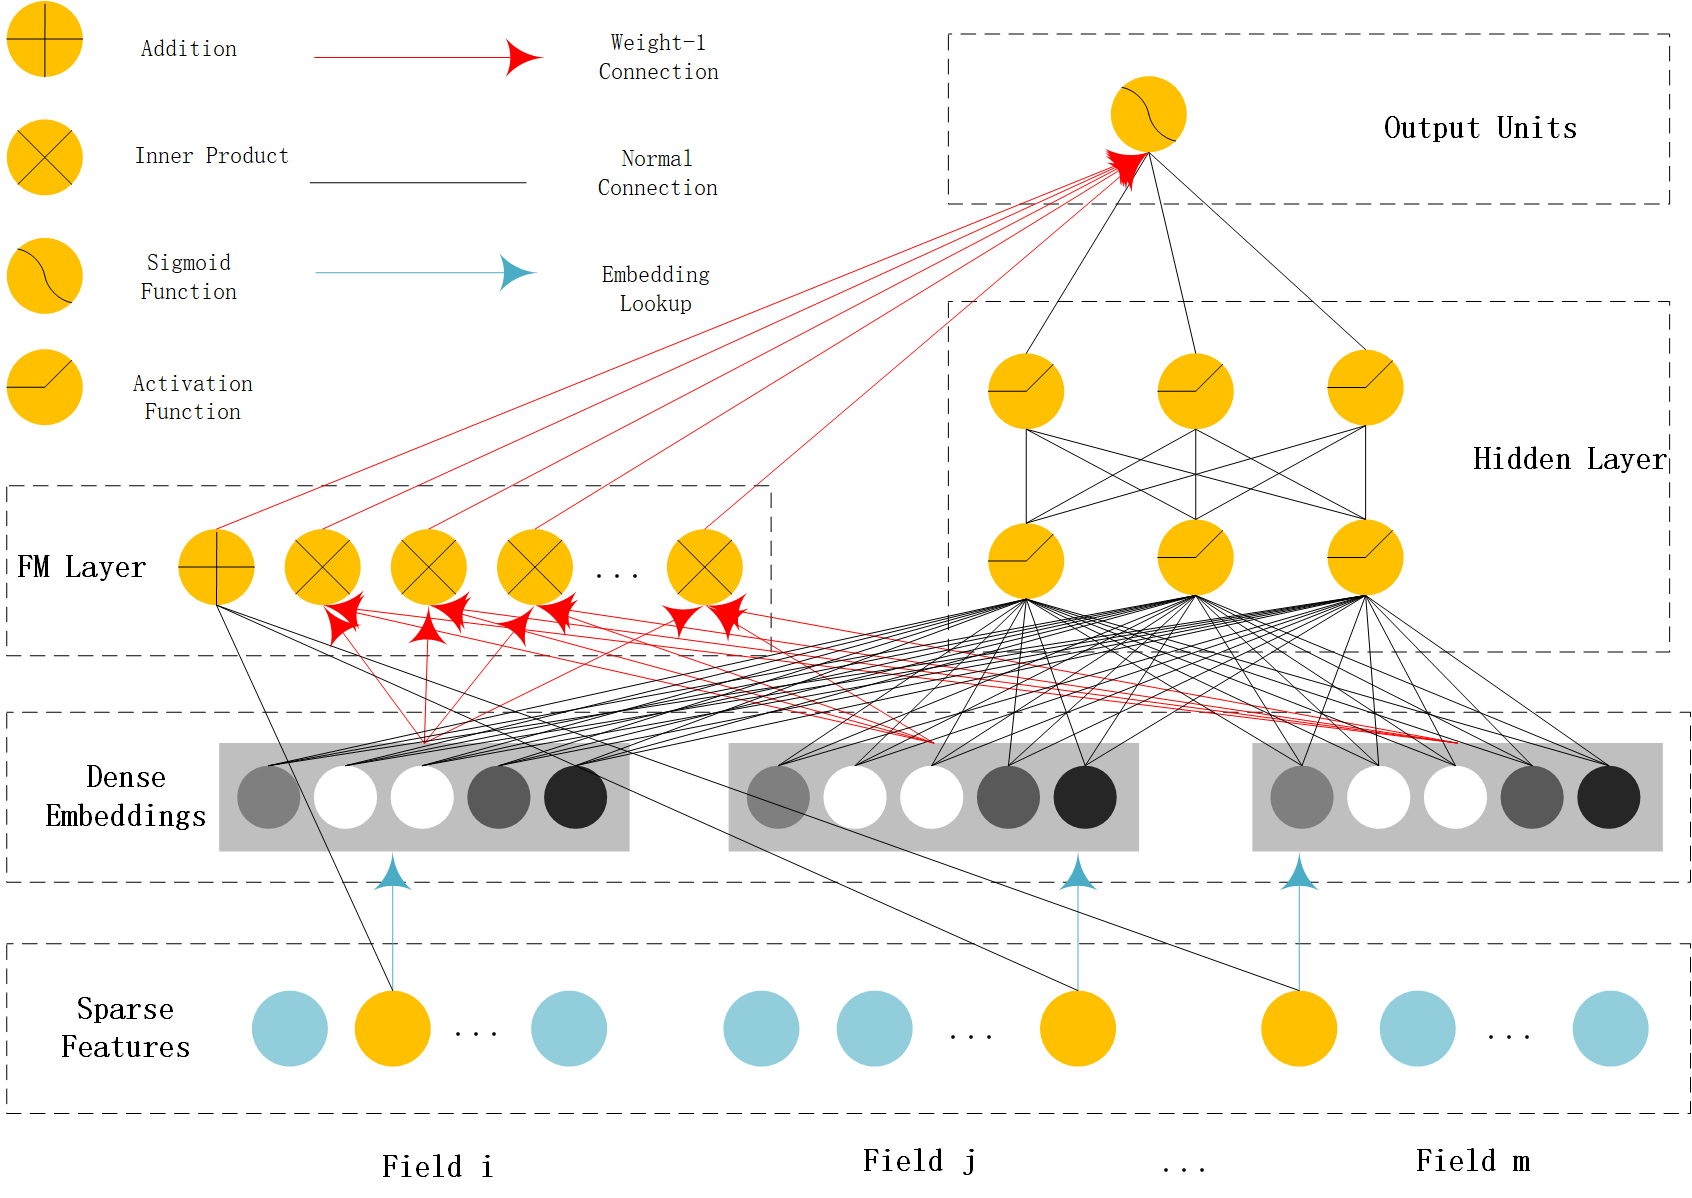
\includegraphics[width=0.95\textwidth]{images/DeepFM.png}
  \caption{DeepFM结构图\cite{DeepFM结构图}}\label{DeepFM结构图} % label 用来在文中索引
\end{figure}

可见DeepFM与Wide \& Deep的框架极为类似,差异在于在Wide部分的特征交叉输入项被替换为FM部分,FM代替Wide部分的手动特征工程构造二阶特征叉乘,从而实现了低阶的自动特征工程。DeepFM的Wide与Deep模块共享相同的由各个Field的one-hot编码横向拼接而成的高维稀疏向量输入;除此以外FM层与NN层共享相同的embedding层,从而降低了模型的复杂度,并且在embedding层训练过程中同时接受低维以及高维特征交互的反馈。在DeepFM的实验中作者对embedding层分别进行了共享与不共享的对比,发现共享效果更优。





FM部分的结构如上,FM对应的输出如下:





DNN部分的结构如下:


